\documentclass{article}

%other packages
\usepackage[a4paper]{geometry}
\usepackage{longtable}
\usepackage{wrapfig}
\setlength\parindent{0pt}
\usepackage{enumitem}
\usepackage[table]{xcolor}
\usepackage{polynom}
\def\scaleint#1{\vcenter{\hbox{\scaleto[3ex]{\displaystyle\int}{#1}}}}
\usepackage{array}
\newcolumntype{C}{>{{}}c<{{}}} % for '+' and '-' symbols
\newcolumntype{R}{>{\displaystyle}r} % automatic display-style math mode 
\usepackage{tabularray}
\usepackage{dcolumn,tabularx,booktabs}

%maths
\usepackage{mathtools}
\usepackage{amsmath}
\usepackage{amssymb}
\usepackage{amsfonts}
\usepackage{autobreak}

%tikzpicture
\usepackage{tikz}
\usepackage{scalerel}
\usepackage{pict2e}
\usepackage{tkz-euclide}
\usepackage{tikz-3dplot}
\usetikzlibrary{calc}
\usetikzlibrary{patterns,arrows.meta}
\usetikzlibrary{shadows}
\usetikzlibrary{external}
\usetikzlibrary{decorations.pathreplacing,angles,quotes}

%pgfplots
\usepackage{pgfplots}
\pgfplotsset{compat=1.18}
\usepgfplotslibrary{statistics}
\usepgfplotslibrary{fillbetween}

\pgfplotsset{
    standard/.style={
    axis line style = thick,
    trig format=rad,
    enlargelimits,
    axis x line=middle,
    axis y line=middle,
    enlarge x limits=0.15,
    enlarge y limits=0.15,
    every axis x label/.style={at={(current axis.right of origin)},anchor=north west},
    every axis y label/.style={at={(current axis.above origin)},anchor=south east}
    }
}

\begin{document}

Math 115 - Week 1, Class 2 - 5 Jan 2024
\hrule

\vspace{10pt}

{\bf{}EXAMPLE} Find the inverse of $f(x)=\sqrt{x-2}$

\vspace{10pt}

Solution 1:

\begin{align*}
\textnormal{Let }y&=\sqrt{x-2}\quad x\geq2,\ y\geq0\\
y^2&=x-2\\
x&=y^2+2\\
x&\leftrightarrow y\\
y&=x^2+2\\
\therefore f^{-1}(x)&=x^2+2\quad y\geq2,\ x\geq0
\end{align*}

It is very important to be cognizant of the fact that line 1 {\bf{}does not} follow from line 2, even though line 2 {\bf{}does} follow from line 1. That is,

\begin{center}
\begin{tabular}{|ll|}
\hline&\\
$\begin{aligned}[t]
\textnormal{If }a&=\sqrt{b}\\
a^2&=b\\
a&\neq\pm\sqrt{b}\\
\end{aligned}$
&
$\begin{aligned}[t]
\textnormal{If }a^2&=b\\
a&=\pm\sqrt{b}\\
a&\neq\sqrt{b}\\
\end{aligned}$\\[4.5em]
\hline
\end{tabular}
\end{center}

Solution 2:

Rotate $f(x)$ $180^\circ$ or $\pi$rad about the line $y=x$ to obtain $f^{-1}(x)$.

\vspace{10pt}

Now we will investigate the concept of continuity, as it pertains to inverse functions. For example, consider the following diagram:

\begin{center}
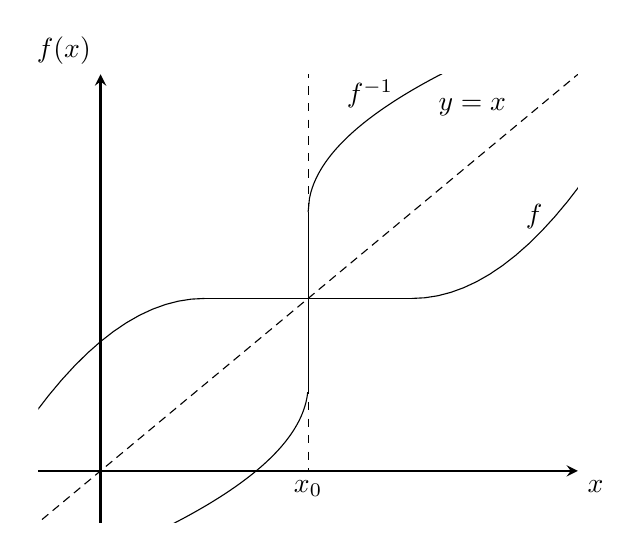
\begin{tikzpicture}
\begin{axis}[
standard,
xmin=0, xmax=2,
ymin=0, ymax=2,
xtick={\empty}, ytick={\empty},
xlabel={$x$}, ylabel={$f(x)$}]
\addplot[densely dashed,domain=-1:3] {x} node[pos=0.75,above left]{$y=x$};
%f(x)
\addplot[domain=-1:0.5] {-(x-0.5)^2+1};
\draw[] (0.5,1) -- (1.5,1);
\addplot[domain=1.5:3] {(x-1.5)^2+1} node[pos=0.25,above]{$f$};
%f^{-1}(x)
\addplot[domain=-1:1,samples=1001] {-(1-x)^(1/2)+0.5};
\draw[] (1,0.47) -- (1,1.5);
\addplot[domain=1:3,samples=301] {(x-1)^(1/2)+1.5} node[pos=0.25,above]{$f^{-1}$};
%discontinuity
\draw[dashed] (1,3) -- (1,0) node[below]{$x_0$};
\end{axis}
\end{tikzpicture}
\end{center}

In this example, the relationship $f$ is indeed a function, and it is indeed continuous. However, the inverse relationship (notice the distinction between the words "relationship" and "function") cannot be a function due to the implications of there being multiple inputs which yield the same output. Recalling that the inverse of a relationship maps the output back to the input. If there are multiple inputs which produce the same output, then the inverse relationship will have an input that corresponds to multiple outputs - which violates the definition of a function.

\vspace{10pt}

In this case, we restrict the domain of $f$ to not include inputs which do not correspond to unique outputs, and define $f^{-1}$ such that the troublesome input is replaced with a jump discontinuity. In this case, the jump discontinuity occurs when $x=x_0$.

\vspace{10pt}

{\bf{}So, a function being continuous does not imply the continuity of its inverse function.}

\vspace{10pt}

Note the following fact;

\begin{center}
\begin{tabular}{|c|}
\hline\\
$f^{-1}(x)$ is continuous if and only if $f(x)$ is $1\to1$ and continuous.\\[1em]
\hline
\end{tabular}
\end{center}

Also, it is worth remembering the general process for determining the inverse function off a relationship:

\begin{enumerate}
\item Let $y=f(x)$
\item Solve for $x$ i.t.o. $y$
\item Interchange $x$ and $y$
\item Let $f^{-1}(x)=y$
\item Verify that $f^{-1}(f(x))=x$ for all $x$ in the domain of $f^{-1}$
\end{enumerate}

{\bf{}EXAMPLE} Find the inverse of $f(x)=\frac{3x+1}{x-2}\quad x\neq2$

\vspace{10pt}

Before we do this, worth mentioning is that you can prove the existence of $f^{-1}$ by proving that $f$ is monotonic. We can differentiate $f$ without the use of the Quotient Rule by converting it from a rational function to a reciprocal function and using the Rower Rule. \[y=\frac{3x+1}{x-2}=\frac{3(x-2)+7}{x-2}=3+\frac{7}{x-2}\Rightarrow y^\prime=\frac{-7}{(x-2)^2}<0\]

So, $f(x)$ is monotonically increasing for all $x$. Therefore $f^{-1}$ exists.

\begin{enumerate}
\item Let $y=\frac{3x+1}{x-2}$
\item Solve for $x$

\begin{align*}
y&=\frac{3x+1}{x-2}\\
y(x-2)&=3x+1\\
yx-3x&=2y+1\\
x(y-3)&=2y+1\\
\Rightarrow x&=\frac{2y+1}{y-3}
\end{align*}

\item $x\leftrightarrow y$ \[\Rightarrow y=\frac{2x+1}{x-3}\]
\item Therefore, $f^{-1}(x)=\frac{2x+1}{x-3}$
\item Verify: $f^{-1}(f(x))=\frac{2\cdot\frac{3x+1}{x-2}+1}{\frac{3x+1}{x-2}-3}=\frac{7x}{x-2}\cdot\frac{x-2}{7}=x$
\end{enumerate}

{\bf{}EXAMPLE} Last class we graphed $\sqrt[3]{1-x^3}$. This class, we will deduce a function which is inversely related to that expression.

\vspace{10pt}

Let $g(x)=\sqrt[3]{1-x^3}$

\begin{enumerate}
\item Let $y=\sqrt[3]{1-x^3}$
\item Solve for $x$

\begin{align*}
y&=\sqrt[3]{1-x^3}\\
x&=\sqrt[3]{1-y^3}
\end{align*}

\item Interchange $x$ and $y$

\[y=\sqrt[3]{1-x^3}\]

\item Therefore, $g^{-1}(x)=\sqrt[3]{1-x^3}$
\item Verify: $f^{-1}(f(x))=\sqrt[3]{1-(\sqrt[3]{1-x^3})^3}=\sqrt[3]{1-(1-x^3)}=x$
\end{enumerate}


\end{document}